\documentclass[UTF8,fontset=fandol]{article}
\title{猫站小报 第 1 期}
\author{猫站小报编辑部}
\date{\today}
\usepackage{ctex}
\usepackage{indentfirst}
\setlength{\parindent}{2em}
\usepackage{listing}
\usepackage{xcolor}
\usepackage{graphicx}
\usepackage{geometry}
\geometry{left=0.3in,right=0.3in,top=0.3in,bottom=0.3in}

\begin{document}
\maketitle
\section{编辑部专版}
\subsection{发刊词}

\noindent
\textbf{各位Kitten作者,Python诗人:} 

编程猫社区一直以来是国内最大的少儿编程社区。2023年以来,官方的不作为使得社区比较为所,社区长期缺乏正经的技术性内容,而我们则选择一种偏传统的方式——报刊。来为编程技术留下一些思考的绿地

\noindent
\textbf{我们的小报分为四部分:}

\begin{itemize}
\item 编辑部专版 - 这里会刊登一些科技界的新闻,社区的时间,编辑部的社论
\item 积木纪元 - 这里会刊登一些优秀的Kitten作品,被官方忽视的优秀作品我们会为你刊登
\item 代码诗篇 - 刊登一些优秀的代码编程作品,官方并不重视Python作品,你可以在这里找到那些被忽视的代码
\item 传火者 - 刊登一些教程类的文章,为了提升全社区的编程水平
\end{itemize}

除了第一部分外,所有部分均接受投稿,编辑们的联系方式可以在各版页脚找到。我们计划每周六在社区出刊,当然,作为一个社区项目,八分靠热情,长时间不出刊也有可能发生,你在我们在社区的帖子之下的跟帖就是对我们最大的支持。

\begin{verbatim}
	print("Hello Codemao Newsletter)
\end{verbatim}
\pagebreak

\section{积木纪元}
\subsection{Quillay聊天室}
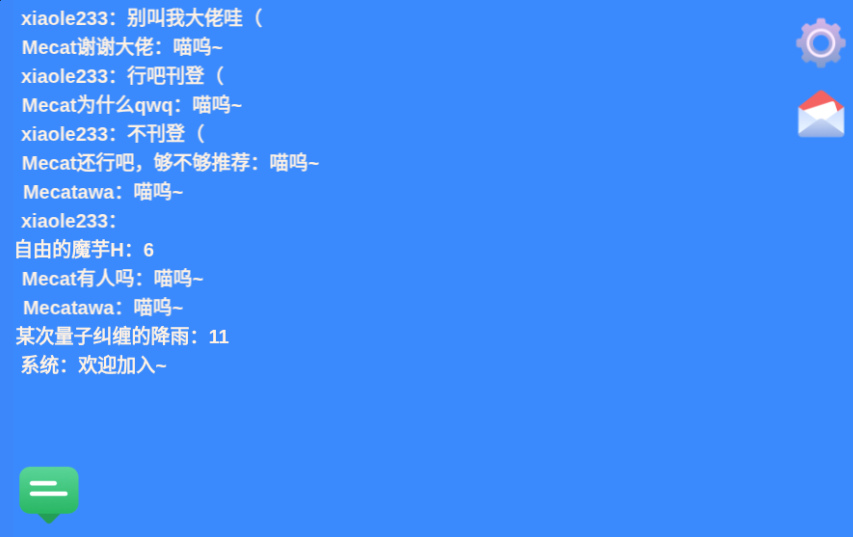
\includegraphics[width=0.5\textwidth]{assets/01/kitten-1.png}

\noindent
\textbf{作者:}Mecat \\
\textbf{ID:}267101361 \\
\textbf{介绍:}一个用KittenN制作的简单的聊天室,目前处于测试阶段 \\
\textbf{编辑评:}刊登这东西的原因是Mecat的死缠烂打
\hfill
\includegraphics[width=0.08\columnwidth]{assets/01/kitten-1-qrc.png}
\subsection{PICKCAT斗地主}
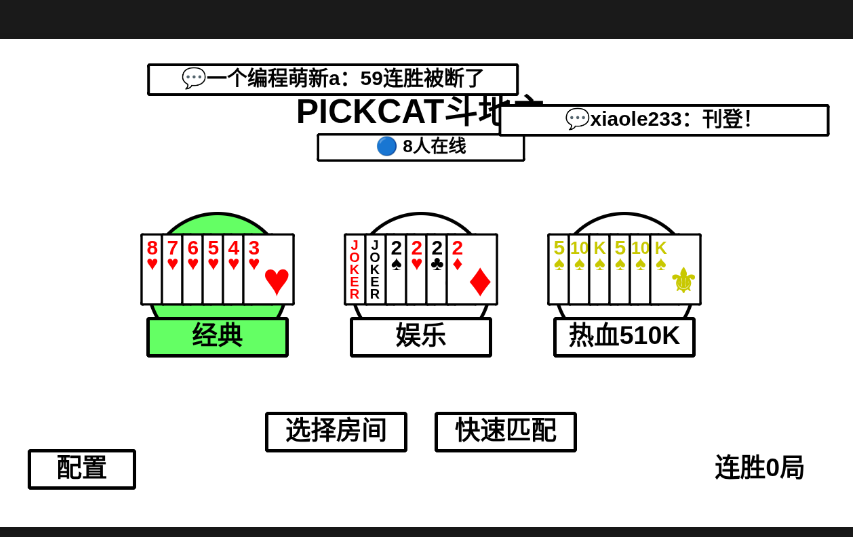
\includegraphics[width=0.5\textwidth]{assets/01/kitten-2.png}

\noindent
\textbf{作者:}钻石awa \\
\textbf{ID:}194885331 \\
\textbf{介绍:}一个用纯画笔公平干净的联机斗地主,据作者所说使用了1w+积木。按回车键还可以发送弹幕。\\
\textbf{编辑评:}编辑部三缺一!
\hfill
\includegraphics[width=0.08\columnwidth]{assets/01/kitten-2-qrc.png}

\pagebreak
\section{代码诗篇}
\subsection{狗皮不通文章生成器}
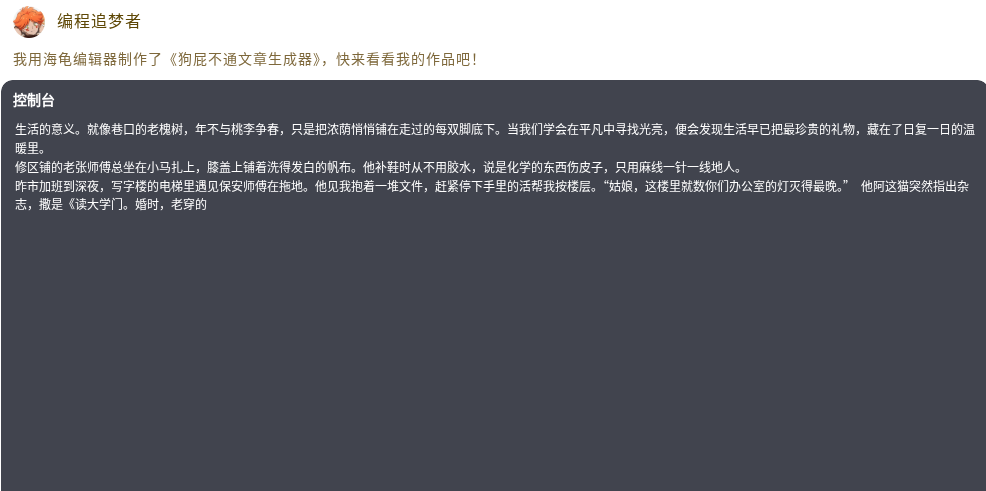
\includegraphics[width=0.5\textwidth]{assets/01/python-1.png}

\noindent
\textbf{作者:}编程追梦者 \\
\textbf{作品ID:}276561815 \\
\textbf{介绍:}使用Python编写的一个作文生成器,生成的作文似乎没有那么狗屁不通?\\
\textbf{编辑评:}追梦者当时跟我说:哈哈,再也不愁作文写不出来了!应该吧(
\hfill 
\includegraphics[width=0.08\columnwidth]{assets/01/python-1-qrc.png}

\subsection{盒子IM刷屏器}
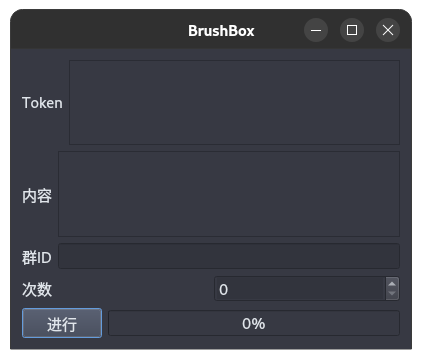
\includegraphics[width=0.5\textwidth]{assets/01/python-2.png}

\noindent
\textbf{作者:}xiaole233 \\
\textbf{Github仓库地址:}Rov-Waff/BrushBox \\
\textbf{介绍:}PyQt编写的一个盒子IM刷屏器,给定你的盒子IM的Token和内容就能刷屏\\
\textbf{编辑评:}编辑卖瓜自卖自夸
\hfill 
\includegraphics[width=0.08\columnwidth]{assets/01/python-2-qrc.png}
\end{document}